\section*{Natural Gas}
\label{sec:natural_gas}
\addcontentsline{toc}{section}{\nameref{sec:natural_gas}}

\subsection{General}
As previously noted, only buildings that indicated natural gas being used \lstinline{NGUSED} were included in the samples for this major fuel use.  Then, one of each pair of predictors with correlations above 0.75 were removed, to avoid model selection issues. Numeric predictors were transformed via BoxCox methodology as well as centered and scaled due to the varying scales and skewness.  Note, no further commentary will be made in the following sections unless it differs from previous sections.

\subsection{Response Analysis}

After filtering for this model's end-use, there are 6662 samples in the data set.  The same transformations were applied to this response variable as electricity. \textit{\hyperref[appendix:natural_gas:response]{Appendix}}

\subsection{Variable Selection - PCA}
RMSE: NA, Rsquared: NA\\
Top 5: \lstinline{NWKER}, \lstinline{EDSEAT}, \lstinline{PBA.14[EDUCATION]}, \lstinline{STRLZR..1[NA]}, \lstinline{PRINTRN}  \textit{\hyperref[appendix:natural_gas:pca]{Appendix}}

\subsection{Variable Selection - PLS}
RMSE: 25929, Rsquared: 0.547\\
Top 5: \lstinline{NWKER}, \lstinline{PRINTRN}, \lstinline{NELVTR}, \lstinline{RFGVNN}, \lstinline{RFGWIN}\\
\\[0.1in]
The Rsquared and RMSE values are significantly poorer than those in the electricity study, which suggests there is either a more complex relationship, or there is greater variance in response, give the available data.  \textit{\hyperref[appendix:natural_gas:pls]{Appendix}}

\subsection{Variable Selection - Random Forest}
RMSE: 27500, Rsquared: 0.748\\
Top 5: \lstinline{SQFTC.8[200K SF - 500K SF]}, \lstinline{NGWATR.2[NO]}, \lstinline{SQFTC.7[100K SF - 200K SF]}, \lstinline{HCBED}, \lstinline{STRLZR.1[YES]} 
\\[0.1in]
The error values are much better for this model, which supports the hypothesis that a good model can be constructed, it will just require the ability to have complex relationships.  \textit{\hyperref[appendix:natural_gas:rf]{Appendix}}

\subsection{Variable Selection - Lasso}
RMSE: NA, Rsquared: NA\\

\subsection{Variable Selection - Forward Selection}
RMSE: 32968, Rsquared: 0.265\\
Top 5: \lstinline{NWKER}, \lstinline{PRINTRN}, \lstinline{NELVTR}, \lstinline{RFGVNN}, \lstinline{RFGWIN}  \textit{\hyperref[appendix:natural_gas:lp]{Appendix}}

\subsection{Variable Selection - Recursive Feature Elimination}
RMSE: 23757, Rsquared: 0.635\\
Top 5: \lstinline{NELVTR}, \lstinline{RFGICN}, \lstinline{NWKER}, \lstinline{HCBED_bin.2[>250]}, \lstinline{PRINTRN}  \textit{\hyperref[appendix:natural_gas:rfe]{Appendix}}

\subsection{Variable Selection - Simple Neural Network}
RMSE: 27866, Rsquared: 0.473\\
Top 5: \lstinline{HCBED_bin.2[>250]}, \lstinline{LINACC.1[YES]}, \lstinline{TVVIDEON_bin.2[>200]}, \lstinline{LAUNDR.3[OFF-SITE SERVICE]}, \lstinline{FACACT.8[HOSPITAL OR OTHER HEALTH CARE COMPLEX]}  
\textit{\hyperref[appendix:natural_gas:snn]{Appendix}}
\newpage
\subsection{Variable Selection - Selected Variable Analysis}
\begin{figure}[h]
\begin{subfigure}{1\textwidth}
\centering
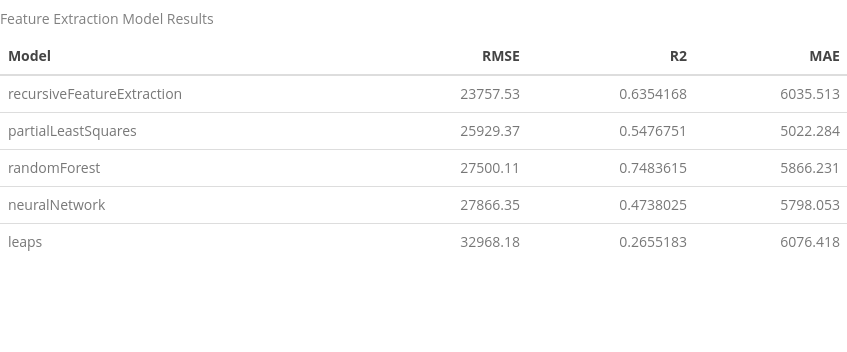
\includegraphics[width=.6\textwidth, height=0.2\textheight]{Images/natural_gas_fe_summary.png}
\end{subfigure}
\begin{subfigure}{1\textwidth}
\centering
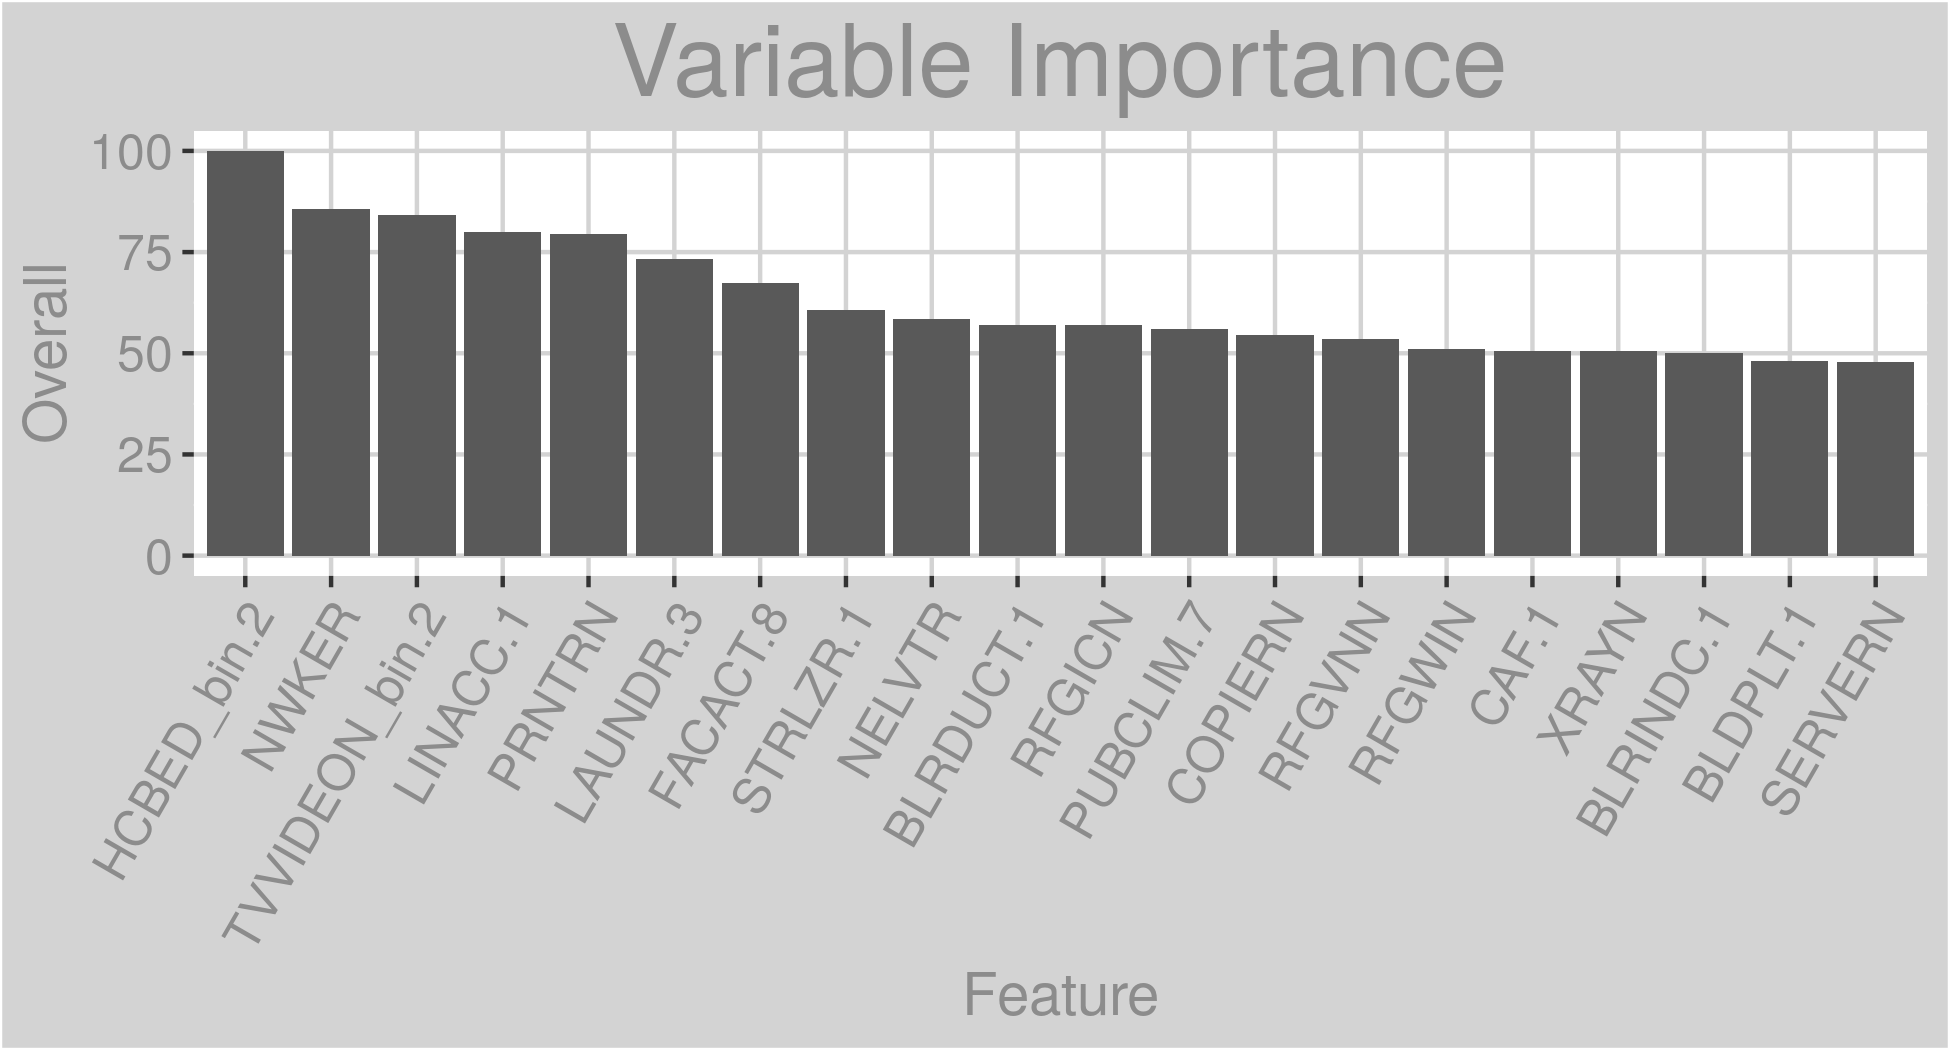
\includegraphics[width=.99\textwidth, height=0.3\textheight]{Images/natural_gas_all_vars.png}
\end{subfigure}
\end{figure}
A number of high importance variables indicated in the electricity analysis are present in this one which indicates there are some attributes that lead to building which have high energy demands for all connected utilities, such as hospitals (\lstinline{HCBED_bin.2[NO]}, \lstinline{FACACT.8[HOSPITAL]}) and refrigerated buildings (\lstinline{RFG*}). Also, it is possible that the models which use these variables may have negative coefficients applied, thus indicating a negative correlation. Additionally, the electricity specific variables (\lstinline{GENUSE}) have dropped significantly. \textit{\hyperref[appendix:electricity:sva]{Appendix}}